\chapter{Evaluation and Findings}
    The fine-tuned classification model is evaluated using standard performance metrics on the reserved test set. To assess generalization, a small handcrafted dataset (see \autoref{subsection:eval_dataset}) is included to reflect real-world variation. Results are reported and analyzed with a focus on metric interpretation, dataset variation, and typical error patterns.

\section{Model Performance}
    The model’s overall accuracy on the test set is 0.966, with matching macro F1 and weighted average. This shows the model performs evenly across both classes. Precision and recall reveal it detects biased cases very well (recall 0.993) but with some false alarms (precision 0.937), meaning a small portion of neutral cases are incorrectly labeled as biased. The confusion matrix confirms this with 10 false positives and only 1 false negative in 325 examples. The false positive rate is 0.057 and the false negative rate is 0.007. Overall, this suggests the model favors detecting bias at the risk of some over-flagging, which fits typical needs for bias detection where missing bias is costlier than false alarms.

        \vspace{0.8em}
        \begin{table}[H]
            \centering
            \begin{tabular}{lccc}
            \toprule
            \textbf{Class} & \textbf{Precision} & \textbf{Recall} & \textbf{F1 Score} \\
            \midrule
            Neutral (0) & 0.994 & 0.943 & 0.968 \\
            Biased (1)  & 0.937 & 0.993 & 0.964 \\
            \bottomrule
            \end{tabular}
            \caption{Per-class precision, recall, and F1 score on the test set}
        \end{table}

        \vspace{0.8em}
        \begin{table}[H]
            \centering
            \begin{tabular}{lc}
            \toprule
            \textbf{Metric} & \textbf{Value} \\
            \midrule
            Accuracy & 0.966 \\
            Macro-average F1 Score & 0.966 \\
            Weighted-average F1 Score & 0.966 \\
            False Positive Rate & 0.057 \\
            False Negative Rate & 0.007 \\
            \bottomrule
            \end{tabular}
            \caption{Overall evaluation metrics on the test set}
        \end{table}

        \begin{figure}[ht]
            \centering
            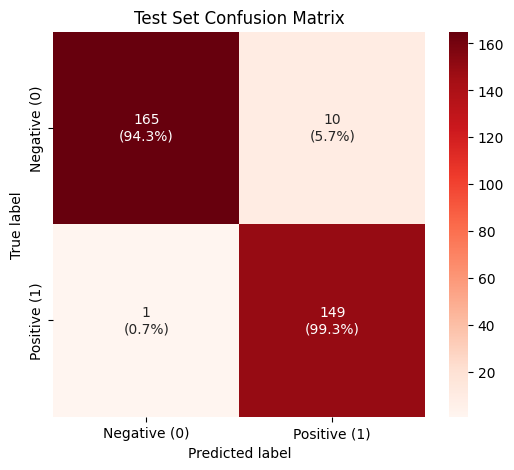
\includegraphics[width=0.75\textwidth]{test_set_confusion_matrix.png}
            \caption[Confusion matrix on the test dataset]{Confusion matrix of the model on the test dataset, showing true vs. predicted labels with counts}
            \label{fig:test_confusion_matrix}
        \end{figure}


\section{Analysis of False Positives and False Negatives}
    False positives and false negatives make up only a small share of the total predictions, but they point to recurring patterns in the model’s errors. These cases were grouped by shared features to enable a structured analysis of likely causes.\footnote{Refer to the appendix for all misclassified examples, including English source texts and German translations.}

    \paragraph{State and Governance Entity Terms}

    Sentences containing political, legal, or governance-related terminology were misclassified the most (6/10 cases). Terms such as president, police officers, heads of state and government, and political leaders were flagged as biased, despite the absence of gendered language in the German translation. These cases suggest that the model may struggle to distinguish between genuinely biased constructions and content related to institutional or geopolitical domains. Another possible explanation is the strong male association of such terms in real-world data, which may influence model behavior through learned co-occurrence patterns \parencite{kroeberItsLongWay2022}.

    \paragraph{Training Dataset Error Causing a False Positive}

    One false positive appears to stem from an inconsistency within the training dataset. The English sentence "[...] or would you go to a surgeon?" was translated as "[...] oder von einem Menschen, der als Chirurg ausgebildet wurde, operieren lassen?". This example originates from the mGeNTE dataset and is labeled as unbiased. The German translation attempts to avoid using "der Chirurg" (m.) by phrasing it as "a person trained as a surgeon," presumably to circumvent the generic masculine form. However, the word "Chirurg" still appears in the translation in its masculine form. The model correctly identified this gendered term and flagged it, despite the label indicating neutrality. From a bilingual perspective, this suggests the model’s detection is valid and points to a labeling inconsistency in the dataset.

    \paragraph{Religious identities}
    
    One false negative involved a sentence concerning the immigration of muslims. "Muslims" was translated using the generic masculine form "Muslime", yet the model failed to flag this instance as biased. 

    To further investigate this issue, the demo was used to test additional cases by replacing the term "Muslims" with other words, summarized in the table below. The evaluation began with other religious terms, followed by "soldiers" to represent a non-religious but contextually relevant group, and concluded with "doctors," a typical example of a generic masculine translation.

        \vspace{0.8em}
        \begin{table}[H]
            \centering
            \begin{tabular}{lc}
            \toprule
            \textbf{Replacement Term} & \textbf{Bias Flag} \\
            \midrule
            Christians & No bias detected (confidence: 0.89) \\
            Jews & No bias detected (confidence: 0.93) \\
            Soldiers & No bias detected (confidence: 0.79) \\
            Doctors & No bias detected (confidence: 0.64) \\
            \bottomrule
            \end{tabular}
            \caption[Bias detection for replacement terms testing religious identity misclassification]{Summary of bias detection results for various replacement terms, showing confidence scores and absence of bias flags.}
        \end{table}
    
    The consistent failure to detect bias across these terms, all translated using the generic masculine form, suggests the issue may stem from the grammatical structure of the sentence or the surrounding military context. Such cases reveal that the model sometimes misses bias for unclear reasons in complex or context-heavy sentences.

    \paragraph{Issues with GFL and Semantically Gendered Terms}

    Two instances were incorrectly flagged as biased due to the use of GFL. The gender-ambiguous terms "specialists" and "recipient" were translated as "Sachkundigen" and "Rezipierende," respectively, both using participial constructions that avoid explicit gender marking. The false detection here reflects insufficient understanding of GFL forms.

    Additionally, one semantically gendered term, "uncle," translated as "Onkel," was flagged as biased, even though the gendered reference is inherent to the original English meaning. In such cases, gender is semantically encoded rather than introduced by translation. The model appears to have difficulty distinguishing inherently gendered terms from translation-induced gender bias.

    These issues are further examined in \autoref{subsection:generalization_performance_on_unseen}.

\section{Generalization performance on unseen data} \label{subsection:generalization_performance_on_unseen}
% eg performance on handcrafted data is lower, likely due to its lexical variation..
% mark any generalizability or consistency issues

    \subsection{Sample Cases}
    % concrete examples of wrong and correct bias flags

